\documentclass[journal,12pt,twocolumn]{IEEEtran}
%
\usepackage{setspace}
\usepackage{gensymb}
%\doublespacing
\singlespacing

%\usepackage{graphicx}
%\usepackage{amssymb}
%\usepackage{relsize}
\usepackage[cmex10]{amsmath}
%\usepackage{amsthm}
%\interdisplaylinepenalty=2500
%\savesymbol{iint}
%\usepackage{txfonts}
%\restoresymbol{TXF}{iint}
%\usepackage{wasysym}
\usepackage{amsthm}
\usepackage{mathrsfs}
\usepackage{txfonts}
\usepackage{stfloats}
\usepackage{steinmetz}
\usepackage{bm}
\usepackage{cite}
\usepackage{cases}
\usepackage{subfig}
%\usepackage{xtab}
\usepackage{longtable}
\usepackage{multirow}
%\usepackage{algorithm}
%\usepackage{algpseudocode}
\usepackage{enumitem}
\usepackage{mathtools}
\usepackage{tikz}
\usepackage{circuitikz}
\usepackage{verbatim}
\usepackage{tfrupee}
\usepackage[breaklinks=true]{hyperref}
%\usepackage{stmaryrd}
\usepackage{tkz-euclide} % loads  TikZ and tkz-base
%\usetkzobj{all}
\usepackage{listings}
    \usepackage{color}                                            %%
    \usepackage{array}                                            %%
    \usepackage{longtable}                                        %%
    \usepackage{calc}                                             %%
    \usepackage{multirow}                                         %%
    \usepackage{hhline}                                           %%
    \usepackage{ifthen}                                           %%
  %optionally (for landscape tables embedded in another document): %%
    \usepackage{lscape}     
\usepackage{multicol}
\usepackage{chngcntr}
%\usepackage{enumerate}

%\usepackage{wasysym}
%\newcounter{MYtempeqncnt}
\DeclareMathOperator*{\Res}{Res}
%\renewcommand{\baselinestretch}{2}
\renewcommand\thesection{\arabic{section}}
\renewcommand\thesubsection{\thesection.\arabic{subsection}}
\renewcommand\thesubsubsection{\thesubsection.\arabic{subsubsection}}

\renewcommand\thesectiondis{\arabic{section}}
\renewcommand\thesubsectiondis{\thesectiondis.\arabic{subsection}}
\renewcommand\thesubsubsectiondis{\thesubsectiondis.\arabic{subsubsection}}

% correct bad hyphenation here
\hyphenation{op-tical net-works semi-conduc-tor}
\def\inputGnumericTable{}                                 %%

\lstset{
%language=C,
frame=single, 
breaklines=true,
columns=fullflexible
}
%\lstset{
%language=tex,
%frame=single, 
%breaklines=true
%}

\begin{document}
%


\newtheorem{theorem}{Theorem}[section]
\newtheorem{problem}{Problem}
\newtheorem{proposition}{Proposition}[section]
\newtheorem{lemma}{Lemma}[section]
\newtheorem{corollary}[theorem]{Corollary}
\newtheorem{example}{Example}[section]
\newtheorem{definition}[problem]{Definition}
%\newtheorem{thm}{Theorem}[section] 
%\newtheorem{defn}[thm]{Definition}
%\newtheorem{algorithm}{Algorithm}[section]
%\newtheorem{cor}{Corollary}
\newcommand{\BEQA}{\begin{eqnarray}}
\newcommand{\EEQA}{\end{eqnarray}}
\newcommand{\define}{\stackrel{\triangle}{=}}
\bibliographystyle{IEEEtran}
%\bibliographystyle{ieeetr}
\providecommand{\mbf}{\mathbf}
\providecommand{\pr}[1]{\ensuremath{\Pr\left(#1\right)}}
\providecommand{\qfunc}[1]{\ensuremath{Q\left(#1\right)}}
\providecommand{\sbrak}[1]{\ensuremath{{}\left[#1\right]}}
\providecommand{\lsbrak}[1]{\ensuremath{{}\left[#1\right.}}
\providecommand{\rsbrak}[1]{\ensuremath{{}\left.#1\right]}}
\providecommand{\brak}[1]{\ensuremath{\left(#1\right)}}
\providecommand{\lbrak}[1]{\ensuremath{\left(#1\right.}}
\providecommand{\rbrak}[1]{\ensuremath{\left.#1\right)}}
\providecommand{\cbrak}[1]{\ensuremath{\left\{#1\right\}}}
\providecommand{\lcbrak}[1]{\ensuremath{\left\{#1\right.}}
\providecommand{\rcbrak}[1]{\ensuremath{\left.#1\right\}}}
\theoremstyle{remark}
\newtheorem{rem}{Remark}
\newcommand{\sgn}{\mathop{\mathrm{sgn}}}
\providecommand{\abs}[1]{\left\vert#1\right\vert}
\providecommand{\res}[1]{\Res\displaylimits_{#1}} 
\providecommand{\norm}[1]{\left\lVert#1\right\rVert}
%\providecommand{\norm}[1]{\lVert#1\rVert}
\providecommand{\mtx}[1]{\mathbf{#1}}
\providecommand{\mean}[1]{E\left[ #1 \right]}
\providecommand{\fourier}{\overset{\mathcal{F}}{ \rightleftharpoons}}
%\providecommand{\hilbert}{\overset{\mathcal{H}}{ \rightleftharpoons}}
\providecommand{\system}{\overset{\mathcal{H}}{ \longleftrightarrow}}
	%\newcommand{\solution}[2]{\textbf{Solution:}{#1}}
\newcommand{\solution}{\noindent \textbf{Solution: }}
\newcommand{\cosec}{\,\text{cosec}\,}
\providecommand{\dec}[2]{\ensuremath{\overset{#1}{\underset{#2}{\gtrless}}}}
\newcommand{\myvec}[1]{\ensuremath{\begin{pmatrix}#1\end{pmatrix}}}
\newcommand{\mydet}[1]{\ensuremath{\begin{vmatrix}#1\end{vmatrix}}}
%\numberwithin{equation}{section}
\numberwithin{equation}{subsection}
%\numberwithin{problem}{section}
%\numberwithin{definition}{section}
\makeatletter
\@addtoreset{figure}{problem}
\makeatother
\let\StandardTheFigure\thefigure
\let\vec\mathbf
%\renewcommand{\thefigure}{\theproblem.\arabic{figure}}
\renewcommand{\thefigure}{\theproblem}
%\setlist[enumerate,1]{before=\renewcommand\theequation{\theenumi.\arabic{equation}}
%\counterwithin{equation}{enumi}
%\renewcommand{\theequation}{\arabic{subsection}.\arabic{equation}}
\def\putbox#1#2#3{\makebox[0in][l]{\makebox[#1][l]{}\raisebox{\baselineskip}[0in][0in]{\raisebox{#2}[0in][0in]{#3}}}}
     \def\rightbox#1{\makebox[0in][r]{#1}}
     \def\centbox#1{\makebox[0in]{#1}}
     \def\topbox#1{\raisebox{-\baselineskip}[0in][0in]{#1}}
     \def\midbox#1{\raisebox{-0.5\baselineskip}[0in][0in]{#1}}
\vspace{3cm}
\title{
SM5083 - BASICS OF PROGRAMMING
	}
\author{ RS Girish - EE20RESCH14005$^{*}$% <-this % stops a space
\thanks{*The author is with the Department
		of Electrical Engineering, Indian Institute of Technology, Hyderabad
		502285 India e-mail:  ee20resch14005@iith.ac.in. All content in this document is released under GNU GPL.  Free and open source.}
	}
\maketitle
\newpage
\tableofcontents
\bigskip
\renewcommand{\thefigure}{\theenumi}
\renewcommand{\thetable}{\theenumi}
\begin{abstract}
This paper contains solution to problem no 5 of Examples III Section of Chapter III of Analytical Geometry by Hukum Chand.
Links to Python codes are available below.  
\end{abstract}
Download python codes at 
\begin{lstlisting}
https://github.com/rsgirishkumar/SM5083/ASSIGNMENT2
\end{lstlisting}
\section{Problem}
The opposite vertices of a square are $\myvec{0\\-1},\myvec{0\\3}$. Find the equations of four sides.
\section{Solution}
Let the given points are indicated as below\\
\begin{align}
\begin{split}
\vec{A} = \myvec{0 \\ -1}, 
\vec{C} = \myvec{0 \\ 3}.\\
\end{split}
\end{align}
Let the unknown vertices are indicated as $ \vec{B},\vec{D}$. The step by step procedure involves
\begin{enumerate}
    \item Find the diagonal $\vec{AC}$.
    \item Find the norm of $\vec{AC}$.
    \item Find the orthogonal of $\vec{AC}$ i.e. $\vec{BD}$ by using orthogonal matrix.
    \item Find the midpoint of $\vec{AC}$.
    \item Using the norm of $\vec{BD}$, find the vertices of $\vec{BD}$.
    \item Form the equations of lines using vertices.
\end{enumerate}
\textbf{Step-1:} Diagonal $\vec{AC}$
\begin{align}
\begin{split}
\vec{AC} = \myvec{0-0\\3+1} = \myvec{0\\4}
\end{split}
\end{align}
\textbf{Step-2:} Norm of $\vec{AC}$
\begin{align}
\begin{split}
\Vert\vec{AC}\Vert = \sqrt{0+4^2} = 4
\end{split}
\end{align}
\textbf{Step-3:} Orthogonal of $\vec{AC}$. i.e, $\vec{BD}$.
\\
Consider an 2x2 orthogonal matrix $\vec{O}$ be $\myvec{0&1\\-1&0}.$
\\
\begin{align}
\begin{split}
\vec{BD} =  \vec{AC} * \vec{O} =  \myvec{0&4}  \myvec{0&1\\-1&0} = \myvec{-4\\0}
\end{split}
\end{align}
\textbf{Step-4:} Midpoint of $\vec{AC}$ or $\vec{BD}$.
\\
\begin{align}
\begin{split}
Midpoint\ \vec{M} = \myvec{0 \\ \frac{(3-1)}{2}} = \myvec{0\\1}
\end{split}
\end{align}
\textbf{Step-5:} Vertices of $\vec{BD}$.
Taking counter-clockwise and norm = 4,
\\
\begin{align}
\begin{split}
\vec{B} = \myvec{\vec{M[0]}-\frac{norm}{2}\\\vec{M[1]}} = \myvec{0-2\\1} = \myvec{-2\\1}\\
\vec{D} = \myvec{\vec{M[0]}+\frac{norm}{2}\\\vec{M[1]}} = \myvec{0+2\\1} = \myvec{2\\1}
\end{split}
\end{align}
\textbf{Step-6:} Line Equations.
Coordinates are
\\
\begin{align}
\begin{split}
\vec{A} = \myvec{0 \\ -1},
\vec{B} =\myvec{-2\\1} ,
\vec{C} = \myvec{0 \\ 3},
\vec{D} =\myvec{2\\1}.
\end{split}
\end{align}
When two coordinates $\myvec{X_1\\ Y_1}, \myvec{X_2 \\Y_2}$ are given, then the line equation is given by 
\begin{align}
\begin{split}
\frac{(Y-Y1)}{(Y2-Y1)} = \frac{(X-X1)}{(X2-X1)}
\end{split}
\end{align}\\
and on comparison with the form ax+by+c=0,\\ \begin{align}
\begin{split}
a= Y_2-Y_1,\\ b=X_1-X_2, \\c=(-(Y_2-Y_1)*X_1)+((X_2-X_1)*Y_1)
\end{split}
\end{align}.\\ 
In Matrix form, $\vec{PT_1} = \myvec{X_1\\Y_1}, \vec{PT_2} = \myvec{X_2\\Y_2}$ and vector \\$\vec{DV_1} = \vec{PT_2 - PT_1} =\myvec{X_2-X_1\\ Y_2-Y_1}$ \\then, 
\begin{align}
\begin{split}
a= \vec{DV_1[1]},\\ b=-\vec{DV_1[0]},\\ c = \myvec{\vec{PT_1[1]}&-\vec{PT_1[0]}} \myvec{\vec{DV_1}.T}
\end{split}
\end{align}
\\
\\
By using the same, the line equation $\vec{AB}$ for points $\vec{A} = \myvec{0\\-1},\vec{B}=\myvec{-2\\1}$ is as follows:
\\
\begin{align}
\begin{split}
\vec{AB} = \myvec{-2\\2}\\
a=2,\ b=2,\\
c=\myvec{-1 & 0} \myvec{-2\\2}=2\\
\end{split}
\end{align}
Line equation for $\vec{AB}$
\begin{align}
\begin{split}
\Rightarrow\ 2x+2y+2=0 \ or \ x+y=-1. \\
\end{split}
\end{align}
In vector form
\begin{align}
\begin{split}
\Rightarrow \myvec{1&1}\ \vec{X}=-1\\
\end{split}
\end{align}
\\
The line equation $\vec{BC}$ for points $\vec{B} = \myvec{-2\\1},\vec{C}=\myvec{0\\3}$ is as follows:
\\
\begin{align}
\begin{split}
\vec{BC} = \myvec{2\\2}\\
a=2,\ b=-2,\\
c=\myvec{1 & 2} \myvec{2\\2}=6\\
\end{split}
\end{align}
Line equation for $\vec{BC}$
\begin{align}
\begin{split}
\Rightarrow\ 2x-2y+6=0 \ or \ x-y=-3. \\
\end{split}
\end{align}
In vector form
\begin{align}
\begin{split}
\Rightarrow \myvec{1&-1}\ \vec{X}=-3
\end{split}
\end{align}
\\
The line equation $\vec{CD}$ for points $\vec{C}=\myvec{0\\3},\vec{D} = \myvec{2\\1}$ is as follows:
\\
\begin{align}
\begin{split}
\vec{CD} = \myvec{2\\-2}\\
a=-2,\ b=-2,\\
c=\myvec{3 & 0} \myvec{2\\-2}=6\\
\end{split}
\end{align}
Line equation for $\vec{CD}$
\begin{align}
\begin{split}
 \Rightarrow\ -2x-2y+6=0 \ or \ x+y=3. \\
\end{split}
\end{align}
In vector form
\begin{align}
\begin{split}
\Rightarrow \myvec{1&1}\ \vec{X}=3
\end{split}
\end{align}
\\
The line equation $\vec{DA}$ for points $\vec{D} = \myvec{2\\1}, \vec{A} = \myvec{0\\-1}$ is as follows:\\
\begin{align}
\begin{split}
\vec{DA} = \myvec{-2\\-2}\\
a=-2,\ b=2,\\
c=\myvec{1 & -2} \myvec{-2\\-2}=2\\
\end{split}
\end{align}
Line equation for $\vec{DA}$
\begin{align}
\begin{split}
\Rightarrow\ -2x+2y+2=0 \ or \ x-y=1. \\
\end{split}
\end{align}
In vector form
\begin{align}
\begin{split}
\Rightarrow \myvec{1&-1}\ \vec{X}=1
\end{split}
\end{align}.
\\
The plotted graph is shown as below.
\begin{figure}[!ht]
    \centering
    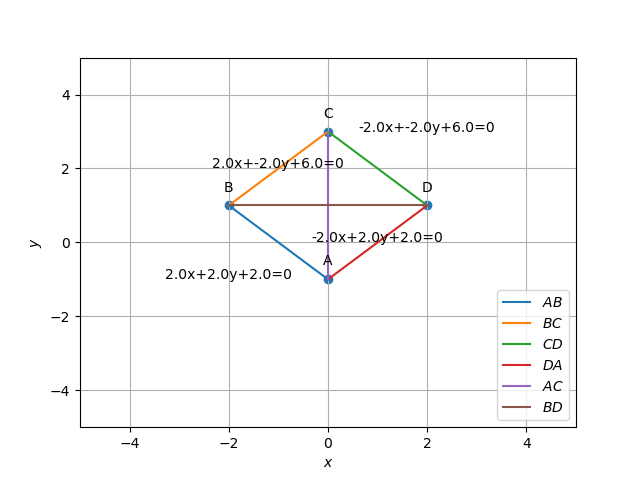
\includegraphics[width=\columnwidth]{assignment2.png}
    \caption{Square ABCD}
    \label{fig:Square ABCD}
\end{figure}
\end{document}